

\documentclass[a4paper,12pt]{article}
%%%%%%%%%%%%%%%%%%%%%%%%%%%%%%%%%%%%%%%%%%%%%%%%%%%%%%%%%%%%%%%%%%%%%%%%%%%%%%%%%%%%%%%%%%%%%%%%%%%%%%%%%%%%%%%%%%%%%%%%%%%%%%%%%%%%%%%%%%%%%%%%%%%%%%%%%%%%%%%%%%%%%%%%%%%%%%%%%%%%%%%%%%%%%%%%%%%%%%%%%%%%%%%%%%%%%%%%%%%%%%%%%%%%%%%%%%%%%%%%%%%%%%%%%%%%
\usepackage{eurosym}
\usepackage{vmargin}
\usepackage{amsmath}
\usepackage{graphics}
\usepackage{epsfig}
\usepackage{subfigure}
\usepackage{fancyhdr}
%\usepackage{listings}
\usepackage{framed}
\usepackage{graphicx}
\usepackage{amsmath}
\usepackage{chngpage}
%\usepackage{bigints}


\setcounter{MaxMatrixCols}{10}
%TCIDATA{OutputFilter=LATEX.DLL}
%TCIDATA{Version=5.00.0.2570}
%TCIDATA{<META NAME="SaveForMode" CONTENT="1">}
%TCIDATA{LastRevised=Wednesday, February 23, 2011 13:24:34}
%TCIDATA{<META NAME="GraphicsSave" CONTENT="32">}
%TCIDATA{Language=American English}

%\pagestyle{fancy}
%\setmarginsrb{20mm}{0mm}{20mm}{25mm}{12mm}{11mm}{0mm}{11mm}
%\lhead{MA4413} \rhead{Mr. Kevin O'Brien}
%\chead{Statistics For Computing}
%\input{tcilatex}

\begin{document}
\begin{center}

\includegraphics[scale=0.65]{images/shieldtransparent2}
\end{center}

\begin{center}
\vspace{1cm}
\large \bf {FACULTY OF SCIENCE AND ENGINEERING} \\[0.5cm]
\normalsize DEPARTMENT OF MATHEMATICS AND STATISTICS \\[1.25cm]
\large \bf {END OF SEMESTER EXAMINATION PAPER 2015} \\[1.5cm]
\end{center}

\begin{tabular}{ll}
MODULE CODE: MA4605 & SEMESTER: Autumn 2015 \\[1cm]
MODULE TITLE: Chemometrics & DURATION OF EXAM: 2.5 hours \\[1cm]
LECTURER: Mr. Kevin O'Brien & GRADING SCHEME: 100 marks \\
& \phantom{GRADING SCHEME:} \footnotesize {60\% of module grade} \\[0.8cm]
EXTERNAL EXAMINER: Prof. J. King & \\
\end{tabular}
\bigskip
\begin{center}
{\bf INSTRUCTIONS TO CANDIDATES}
\end{center}

{\noindent \\ Scientific calculators approved by the University of Limerick can be used. \\
Formula sheet and statistical tables areprovided at the end of the exam paper.\\
Students must attempt any 4 questions from 5.}
\newpage



% - Section 1 Inference Procedures
        % a. Parametric
        % b. Non Parametric
% - Section 2 Linear Models
        % a. SLR
        % b. MLR
% - Section 3 Linear Models
        % a. Robust Regression
        % b. AIC
% - Section 4 Statistical Process control
        % a. Control Limits
        % b. Theory Questions
        % c. Interpreting Charts
        % d. CUSUM and ARL
% - Section 5 Experimental Design 1
        % a. Definitions for ED
        % b. One Way ANOVA
% - Section 6 Experimental Design 2
        % a.
        % b.


\subsection*{Question 1. (25 marks) Inference Procedures and Distributional Testing}
\subsubsection*{Question 1 Part A (15 Marks)}
% Clincal 

A test of a specific blood factor has been devised such that, for adults in Western Europe, the test score is normally distributed with mean 100 and standard deviation 10. A clinical research organization is carrying out research on the blood factor levels for sufferers of a particular disease.  

\begin{itemize}
\item A study has obtained the following test scores for 14 randomly selected patients suffering from the disease in Ireland 
\[ \{118, 116, 109, 105, 103, 111, 139, 117, 107, 105, 125,  99, 106, 103\}\]

\item A similar study has obtained the following test scores for 14 randomly selected patients suffering from the disease in Denmark.
\[\{120, 140, 112, 109, 114, 116,  99, 108, 109, 111, 109, 131, 117, 101\}\]

\end{itemize}

% The variance of both data sets are equal. 
% You may assume that both data sets are normally distributed.

%===============================%
% 1. outliers
% 3. variance
% 
%===============================%

\noindent The following blocks of \texttt{R} code (i.e. blocks A to E) are based on the data for this assessment. Write a short report on your conclusion for this assessment. \\ \bigskip

\noindent \textit{\textbf{Marking Scheme}: Either 2 or 3 Marks will be awarded for a correct interpretation of each code segment, for a total of 12 Marks. Remember to state the null and alternative hypotheses when relevant. 3 Marks will also be award for an overall conclusion. }

\begin{framed}
\noindent \textbf{Block A} (3 Marks) 

%================================%

	\begin{verbatim}
	> grubbs.test(X)
	
	Grubbs test for one outlier
	
	data:  X
	G = 2.56990, U = 0.45291, p-value = 0.01748
	alternative hypothesis: highest value 139 is an outlier
	
> grubbs.test(Y)

Grubbs test for one outlier

data:  Y
G = 2.17410, U = 0.66387, p-value = 0.1486
alternative hypothesis: highest value 131 is an outlier

	\end{verbatim}
\end{framed}
%=========================================================================%

	\begin{framed}
\noindent 	\textbf{Block B} (2 Marks)
	\begin{verbatim}
	> shapiro.test(X)
	
	Shapiro-Wilk normality test
	
	data:  X
	W = 0.87633, p-value = 0.05153
	
	
	
> shapiro.test(Y)

Shapiro-Wilk normality test

data:  Y
W = 0.92341, p-value = 0.1914

	\end{verbatim}
\end{framed}
%===========================================================%

	\begin{framed}
\noindent 	\textbf{Block C} (2 Marks)
	\begin{verbatim}
> var.test(X,Y)

F test to compare two variances

data:  X and Y
F = 2.3808, num df = 13, denom df = 15, p-value = 0.1107
alternative hypothesis: true ratio of variances is not equal to 1

95 percent confidence interval:
0.8139616 7.2677776

sample estimates:
ratio of variances 
2.38076 


	\end{verbatim}
\end{framed}
%======================================================%
\newpage
	\begin{framed}
\noindent \textbf{Block D} (3 Marks)
	\begin{verbatim}
> t.test(X,Y,var.equal=TRUE)

Two Sample t-test

data:  X and Y
t = -1.3471, df = 28, p-value = 0.1888
alternative hypothesis: true difference in means is not equal to 0

95 percent confidence interval:
-10.982656   2.268371

sample estimates:
mean of x mean of y 
111.6429  116.0000 
	
	
	
	
> t.test(X,Y,var.equal=FALSE)

Welch Two Sample t-test

data:  X and Y
t = -1.3096, df = 21.764, p-value = 0.204
alternative hypothesis: true difference in means is not equal to 0

95 percent confidence interval:
-11.261465   2.547179

sample estimates:
mean of x mean of y 
111.6429  116.0000 
	\end{verbatim}
\end{framed}
\newpage

\begin{framed}
\textbf{Block E}
\begin{verbatim}
> wilcox.test(X,Y)

Wilcoxon rank sum test with continuity correction

data:  X and Y
W = 68, p-value = 0.06999
alternative hypothesis: true location shift is not equal to 0

\end{verbatim}	
\end{framed}
%==========================================================%
\newpage
\subsubsection*{Question 1 Part B (4 Marks)}
Numeric Transformations, such as logarithmic transformation, are often used in statistical analysis as an approach for dealing with non-normal data.
\begin{itemize}
%	\item[(i)] (1 Marks) Discuss the importance of numeric transformations, such as logarithmic transformation, in Statistics.
%	\item[(ii)] Describe the process of transformations
	\item[(i.)] (1 Marks) Describe the purpose of Tukey's Ladder (referencing direction and relative strength).
	\item[(ii.)] (2 Marks) Give two examples of a transformation for various types of skewed data (i.e. an example for both types of skewness).
	\item[(iii.)] (1 Marks) Discuss the limitations of numeric transformations.
\end{itemize}

\subsubsection*{Question 1 Part C (6 Marks)}

%\subsubsection*{Part A : Outliers}
\begin{itemize}
	\item[(i.)] (3 Marks) Provide a brief description for three tests from the family of Grubb's  Outliers Tests. Include in your description a statement of the null and alternative hypothesis for each test, any required assumptions and the limitations of these tests.
	\item[(ii.)] (3 Marks) Showing your working, use the Dixon Q Test to test the hypothesis that the maximum value of the following data set is an outlier.
	\[ 19,22,23,24,25,26,29,38\]
\end{itemize}	


\newpage



\subsection*{Question 2. (25 marks) Regression Models }
%--------------------------------------------------------------------------------------------------------%
\subsubsection*{Question 2 Part A (8 Marks)}
In an experiment to determine hydrolysable tannins in plants by absorption spectroscopy, the following results from ten samples were obtained and are tabulated below. A simple linear regression model, predicting absorbance values using concentration as the independent variable, was fitted to the data. The scatterplot is depicted below.
%%Absorbance= c(0.084, 0.183, 0.326, 0.464, 0.643, 0.707, 0.717, 0.734 ,0.749 ,0.732) ;
%%Concentration= c(0.123, 0.288, 0.562, 0.921, 1.420, 1.717, 1.921, 2.137 ,2.321, 2.467) ;
%%plot(Concentration,Absorbance,pch=18,col="red",font.axis=2,font.lab=2)
%%abline(coef(lm(Absorbance~Concentration)))

%%Conc.Squared = (Concentration^2)
%%Conc.Cubed = (Concentration^3)
%%ModelA = lm(Absorbance~Concentration)
%%ModelB = lm(Absorbance~Concentration+Conc.Squared)
%%ModelC = lm(Absorbance~Concentration+Conc.Squared+Conc.Cubed)
\begin{center}
	\begin{tabular}{|c||c|c|c|c|c|}
		\hline
		%  % after \\: \hline or \cline{col1-col2} \cline{col3-col4} ...
		Sample & 1 & 2 & 3 & 4 & 5 \\ \hline
		Absorbance & 0.084& 0.183& 0.326& 0.464& 0.643\\
		Concentration & 0.123& 0.288& 0.562& 0.921& 1.420\\ \hline
		Sample & 6 & 7 & 8 & 9 & 10 \\ \hline
		Absorbance & 0.707& 0.717& 0.734 &0.749 &0.732\\
		Concentration & 1.717& 1.921& 2.137 &2.321&2.467\\
		\hline
	\end{tabular}
\end{center}
\begin{center}
	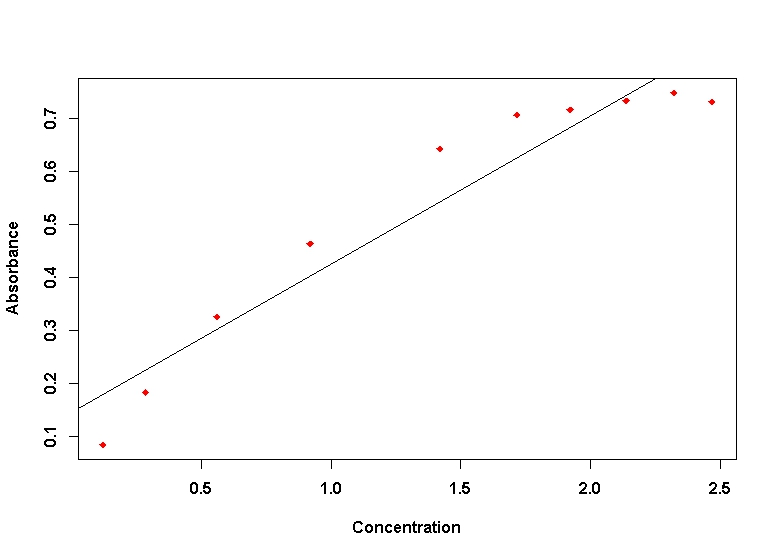
\includegraphics[scale=0.45]{image/ExamQ3plot}
\end{center}
\begin{itemize}
	\item[(i.)] (1 marks) Is the simple linear regression model approach suitable for this study? Explain your answer with reference to the scatter-plot.
	\item[(ii.)] (3 marks) Two polynomial models were also fitted to the data. Description of all three fitted models are found in the three blocks of \texttt{R} code on the following pages. The \emph{Akaike information criterion} is listed, for each of the three fitted models. Write down the regression equations of each of the three models.
	\item[(iii.)] (2 marks) Specify which one of the models you would use. Justify your answer with appropriate statistical values.
	\item[(iv.)] (2 marks) Using the best fitting model, predict a value for absorbance when the concentration level is 1.2 $mg/ml$.

\end{itemize}


%
%
%
%\item[(d)] Two polynomial models were also fitted to the data. Description of all three fitted models are found in the three blocks of \texttt{R} code below. The \emph{Akaike information criterion} is also listed, for each of the three fitted models.
%\begin{itemize}
%\item[i.] (4 marks) Write down the regression equation for each of the three linear models.
%\item[ii.] (2 marks) Based on the \emph{Akaike information criterion}, which fitted model can be assumed to be the best fit of the three candidate models.

%\end{itemize}
%\newpage

	
	\begin{framed}
\noindent \textbf{Model 1}
		\begin{verbatim}
		> summary(Model1)
		Call:
		lm(formula = Absorb ~ Conc)
		...
		Coefficients:
		Estimate Std. Error t value Pr(>|t|)
		(Intercept)    0.14412    0.04721   3.053   0.0158 *
		Concentration  0.28088    0.02930   9.586 1.16e-05 ***
		---
		Signif. codes:  0 �***� 0.001 �**� 0.01 �*� 0.05 �.� 0.1 � � 1
		
		Residual standard error: 0.07584 on 8 degrees of freedom
		Multiple R-squared: 0.9199,     Adjusted R-squared: 0.9099
		F-statistic: 91.89 on 1 and 8 DF,  p-value: 1.163e-05
		>
		>
		>AIC(Model1)
		[1] -19.4343
		\end{verbatim}
	\end{framed}
	
	\begin{framed}
\noindent	\textbf{Model 2}
		\begin{verbatim}
		> summary(Model2)
		Call:
		lm(formula = Absorb ~ Conc + Conc.Squared)
		...
		Coefficients:
		Estimate Std. Error t value Pr(>|t|)
		(Intercept)    0.006582   0.008013   0.821    0.439
		Concentration  0.642935   0.015568  41.299 1.27e-09 ***
		Conc.Squared  -0.140573   0.005894 -23.851 5.79e-08 ***
		---
		Signif. codes:  0 �***� 0.001 �**� 0.01 �*� 0.05 �.� 0.1 � � 1
		
		Residual standard error: 0.008939 on 7 degrees of freedom
		Multiple R-squared: 0.999,      Adjusted R-squared: 0.9987
		F-statistic:  3592 on 2 and 7 DF,  p-value: 2.879e-11
		>
		>
		> AIC(Model2)
		[1] -61.5338
		\end{verbatim}
	\end{framed}
	
	\newpage
	\begin{framed}
\noindent \textbf{Model 3}
		\begin{verbatim}
		> summary(Model3)
		
		Call:
		lm(formula = Absorb ~ Conc+ Conc.Squared + Conc.Cubed)
		...
		...
		Coefficients:
		Estimate Std. Error t value Pr(>|t|)
		(Intercept)    0.013712   0.011629   1.179   0.2830
		Concentration  0.608682   0.042825  14.213 7.58e-06 ***
		Conc.Squared  -0.108186   0.038088  -2.840   0.0296 *
		Conc.Cubed    -0.008196   0.009518  -0.861   0.4223
		---
		Signif. codes:  0 �***� 0.001 �**� 0.01 �*� 0.05 �.� 0.1 � � 1
		
		Residual standard error: 0.009109 on 6 degrees of freedom
		Multiple R-squared: 0.9991,     Adjusted R-squared: 0.9987
		F-statistic:  2306 on 3 and 6 DF,  p-value: 1.422e-09
		>
		>
		> AIC(Model3)
		[1] -60.69903
		\end{verbatim}
	\end{framed}
\newpage
%-------------------------------Start of Question 2B%
%\item[(b)](6 marks)
%The scatter-plot contains the regression line for the fitted model. Three diagnostic plots, used to assess the suitability of the fitted model, are presented on the following pages. Provide a brief interpretation for each of the three diagnostic plots described in part(a). The scatter-plot for the data is also presented.

%\begin{center}
%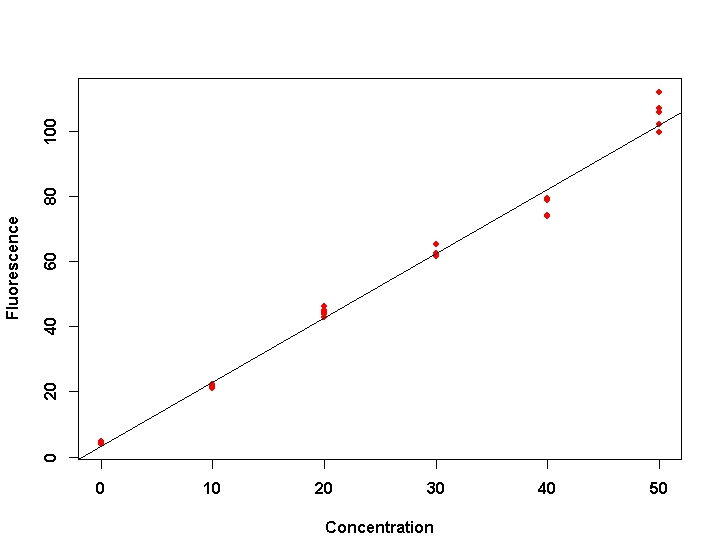
\includegraphics[scale=0.60]{ExamQ2plot2}
%\end{center}
%\newpage
%\begin{center}
%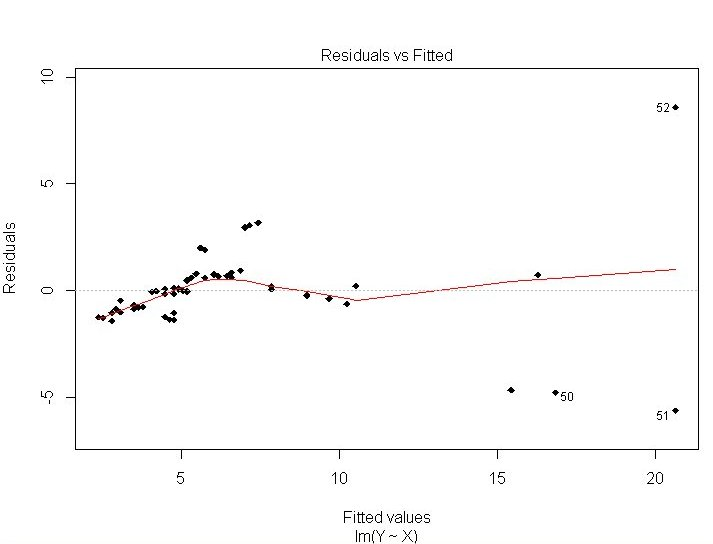
\includegraphics[scale=0.55]{ExamQ2diag1}
%\end{center}
%
%\begin{center}
%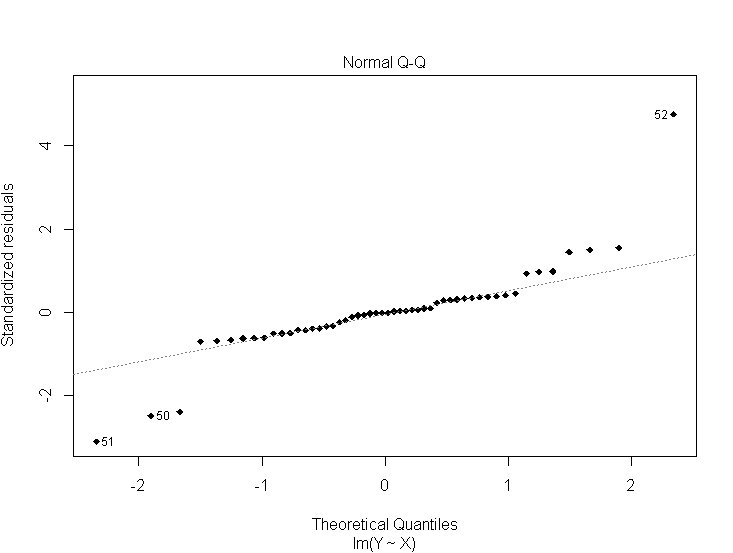
\includegraphics[scale=0.55]{ExamQ2diag2}
%\end{center}
%
%\begin{center}
%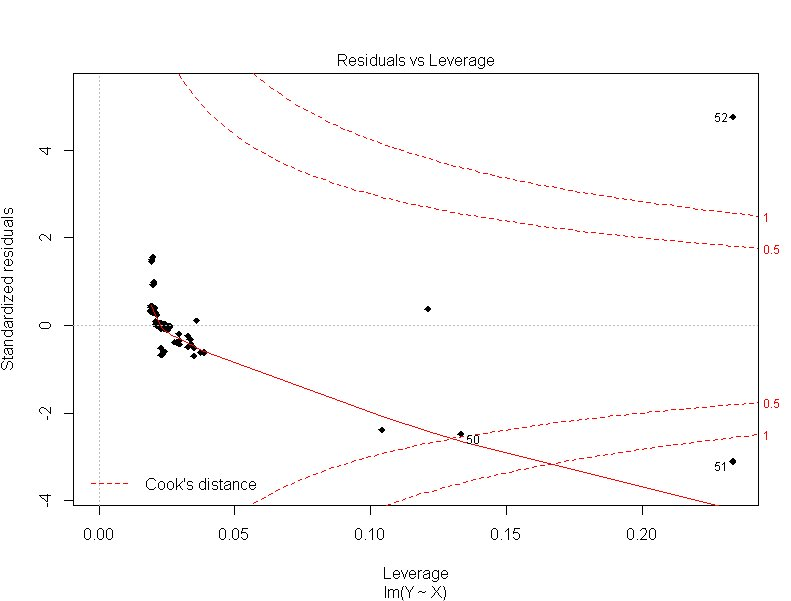
\includegraphics[scale=0.55]{ExamQ2diag3}
%\end{center}

%%-------------------------------End  of Question 2B%
%\newpage
%\subsubsection*{Question 2 Part B (10 Marks)}	
% Complete the following \textit{Analysis of Variance} Table for a simple linear regression model based on the data provided. The required values are indicated by question marks.
%\begin{center}
%	\begin{tabular}{|c|c|c|c|c|c|} \hline
%		& Df & 	Sum Sq &	Mean Sq &	F value &   	Pr($>$F)    \\ \hline
%		Regression &  ? &	9160239 &	? &	 ? &	$< 2.2e^{-16}$ \\ \hline
%		Error  & 50 &	2134710 &  	?   &            &       \\ \hline
%		Total  & ?  &	? &  	42694   &            &       \\ \hline
%	\end{tabular} 
%\end{center}
%
%Once you have completed this table, compute the following
%\begin{itemize}
%	\item (1 Mark) The Pearson correlation coefficient for the response variable Y and the predictor variable X.
%	\item (1 Mark) The sample standard deviation of the response variable Y.
%\end{itemize}


\subsubsection*{Question 2 Part B (7 Marks)}

% \subsection*{Q9.Robust Regression}
%Write a brief explanation of how robust regression differs from linear models computed using the \emph{Ordinary Least Squares method}, making reference to one particular weighting method only. Provide a description on how this weighting method works.


In certain circumstances, Robust Regression may be used in preference to Ordinary Least Squares Regression. Answer the following questions relating to Robust Regression. 

\begin{itemize}
	\item[(i.)] (1 Mark) Describe what these circumstances might be.
	\item[(ii.)] (1 Mark) State one difference between OLS and Robust regression techniques, in terms of computing regression equations.
	\item[(iii.)] (2 Marks) Explain the process of Huber Weighting for Residuals, stating the algorithm used to compute weightings.
	\item[(iv.)] (3 Marks) Suppose that Huber Weighting, with a tuning constanct of $k=13.45$, was applied to the observations 
	tabulated below. What would be the outcome of the procedure for each case. 
\end{itemize}
\begin{center}
	\begin{tabular}{|c|c|}
		\hline
		Observation & Residual \\ 
		$i$  & $e_i$ \\ \hline
		11 & -9.07 \\ \hline 
		14 & 14.54 \\ \hline
		18 & 22.91 \\ \hline
	\end{tabular} 
\end{center}

\subsubsection*{Question 2 Part C (10 Marks)}
%The following scatterplot
%\begin{figure}[h!]
%\centering
%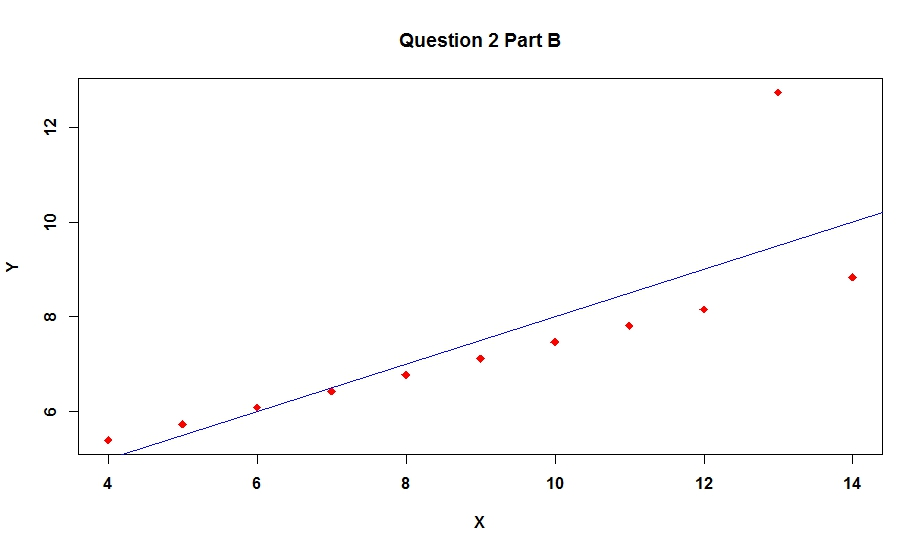
\includegraphics[width=0.8\linewidth]{images/ExamQ2diagnostics}
%\end{figure}
\begin{itemize}
\item[(i.)] (1 Marks) Explain the term ``Influence" in the context of linear regression models. Support your answer with sketches.
\item[(ii.)] (1 Marks) Explain the  term ``Cook's Distance" in the context of linear regression models. 
\item[(iii.)] (2 Marks) The following plot is the \textit{Residual vs Fitted} plot, the first of \texttt{R}'s diagnostic plots for linear models. Briefly describe how to interpet this plot. What is your conclusion?
\begin{figure}[h!]
	\centering
	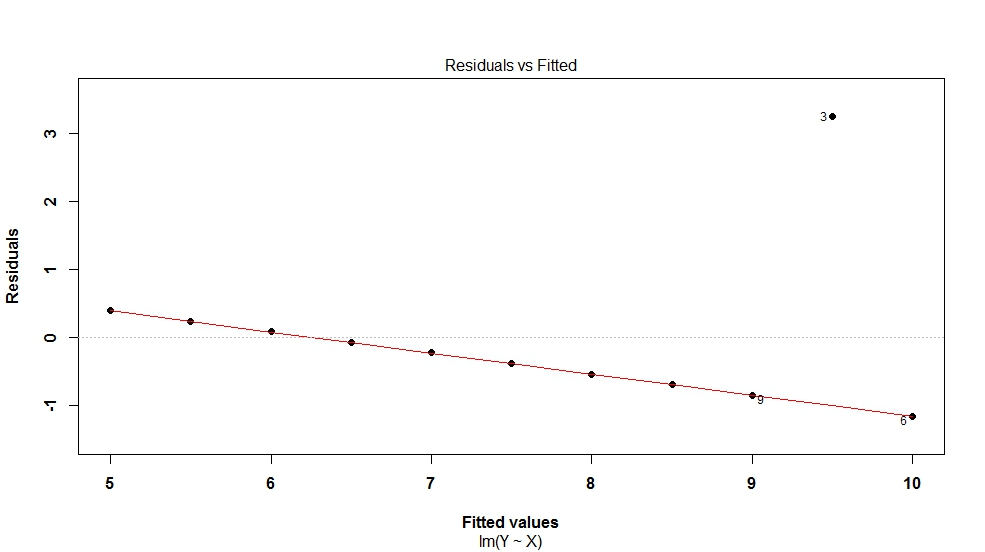
\includegraphics[width=0.8\linewidth]{images/ExamQ2diag1anscombe}
\end{figure}
\newpage
\item[(iv.)] (2 Marks) Explain the term ``Heteroscedascity" in the context of linear regression models. Support your answer with sketches.
\item[(v.)] (1 Mark) The Non-constant Variance Score Test was carried out to test for Heteroscedascity. The output is depicted below. State your conclusion to the following procedure.

\begin{framed}
	\begin{verbatim}
	> ncvTest(ModelQ2)
	Non-constant Variance Score Test 
	Variance formula: ~ fitted.values 
	Chisquare = 7.585432    Df = 1     p = 0.005884187
	\end{verbatim}
\end{framed}
%
%\item[(vi)] (3 Marks) Outliers Test
%\begin{framed}
%	\begin{verbatim}
%	> outlierTest(ModelQ2)
%	rstudent unadjusted p-value Bonferonni p
%	3 1203.539         2.5441e-22   2.7985e-21
%	\end{verbatim}
%\end{framed}

\item[(vi.)] (2 Marks)  The Durbin Watson Test was carried out to test for Autocorrelation. Briefly describe autocorrelation. You may support your answer with sketches.
\item[(vii.)] (1 Mark) State your conclusion to the following procedure.
\begin{framed}
	\begin{verbatim}
	> durbinWatsonTest(ModelQ2)
	lag Autocorrelation D-W Statistic p-value
	1     -0.08428163      2.143578   0.806
	Alternative hypothesis: rho != 0
	\end{verbatim}
\end{framed}

\end{itemize}


%-------------------------------End  of Question 2B%






\newpage






%\item[(b)]


%---------------------%



%\item[(c)] (6 marks)
% 







%%-------------------------------------%
%\subsection*{Question 3. (20 marks) Multiple Linear Regression Models }
%\begin{itemize}
%
%\item[(a)] Explain the following terms:
%\begin{itemize}
%\item[i.] (2 marks) Over-fitting,
%\item[ii.] (2 marks) Multicollinearity,

%\end{itemize}
%\item[(b)] Answer the following questions related to model selection techniques for linear models.
%\begin{itemize}
%\item[i.] (2 marks) Explain why the adjusted $R^2$ value may differ in value from the corresponding multiple $R^2$ value for the same fitted model.
%\item[ii.] (2 marks) Explain how the \emph{Akaike information criterion} would used to compare two models fitted for the same data.
%\end{itemize}
%

%
%
%%\end{document}
%--------------------------------------------------------%

% Definitions
% One Way ANOVA
% Checking Assumptions

\newpage
\large\subsection*{Question 3. (25 marks) Experimental Design }
\subsubsection*{Question 3 Part A (15 Marks)}
%
%\subsection*{Water Nitrate (One Way ANOVA MA4605)}

Three investigators, A, B and C, performed six determination of nitrate in water using the same procedure. The results in $\mu$M were:

% Investigator 1 Investigator 2 Investigator 3

\begin{center}
\begin{tabular}{|c|c|c|} \hline
A  &  B   & C \\ \hline \hline
6.7 & 6.3 & 6.8 \\ \hline
6.8 & 6.2 & 6.9 \\ \hline
6.5 & 6.1 & 7.1 \\ \hline
6.8 & 6.3 & 6.9 \\ \hline
6.9 & 6.5 & 7.2 \\ \hline
7.1 & 6.4 & 7.1 \\ \hline
\end{tabular} 
\end{center}
\noindent We are also given the summmary statistics for each of the three investigators, as well as for the samples combined.
\begin{center}
\begin{tabular}{|c|c|c|}
	\hline  & Sample Mean & Sample Variance \\ 
	\hline A & 6.8 & 0.040 \\ 
	\hline B & 6.3 & 0.020 \\ 
	\hline C & 7 & 0.024 \\ 
	\hline Overall & 6.7 & 0.1164 \\ 
	\hline 
\end{tabular} 
\end{center}
\noindent An analysis of variance procedure is used to determine if there is a significant difference between the mean of the determinations made by the three investigators.

% The following output is obtained in R and presented below.

%investigator <- c(6.7, 6.8, 6.5, 6.8, 6.9, 7.1, 6.3, 6.2, 6.1, 6.3, 6.5, 6.4, 
%6.8, 6.9, 7.1, 6.9, 7.2, 7.1)
%A <- investigator[1:6]
%B <- investigator[7:12]
%C <- investigator[13:18]
%
%
%
%group <- factor(rep(1:3,each=6))
%
%aov(investigator~group)
%
%Analysis of Variance Table
%
%Response: investigator

%Df SumSq MeanSq Fvalue Pr(>F)
%
%group ? 1.42333 ? ? 3.133e-05
%
%Residuals 15 ? ?
%
%Total ? 1.9

The following questions will result in the completion of the ANOVA Table on the next page. The $p-$value is already provided.
\begin{itemize}
	\item[(i.)](3 Marks) Compute the Between Groups Sum of Squares. (Show your workings.)
	\item[(ii.)](3 Marks) Compute the Within Groups Sum of Squares.(Show your workings.)
	\item[(iii.)](2 Marks) Compute the Total Sum of Squares. (Show your workings).
	\item[(iv.)] (2 Marks) State the degrees of freedom for the ANOVA Tables
	\item[(v.)] (1 Marks) Compute the Mean Square values.
	\item[(vi.)] (1 Marks) Compute the test Statistic for this procedure (i.e. the F-value.)
	\item[(vii.)] (3 Marks) This analysis is used to assess if there is any difference between the mean determinations made by the three investigators. What is your conclusion? Clearly state the null and alternative hypothesis.
\end{itemize}
%================================================================================ %
\begin{center}
	\begin{tabular}{|c||c|c|c|c|c|}
		\hline Source & DF & SS & MS & F & p-value \\ \hline 
		\hline Between & \phantom{mak} ? \phantom{mak}  & \phantom{mak} ? \phantom{mak}  & \phantom{mak} ? \phantom{mak}  & \phantom{mak} ? \phantom{mak}  &  $8.9\times 10^{-06}$ \\ 
		\hline Within &  ? & ? & \phantom{mak} ? \phantom{mak}  &  &  \\ 
		\hline \hline Total & ? & ? &  &  &  \\ 
		\hline 
	\end{tabular}
\end{center} 
%===================================================================================================== %
\newpage
%\subsubsection*{Question 4 Part B (10 Marks)}
%
%
%
%
%The \texttt{R} code and graphical procedures, below and on the following page, are relevant to checking whether the underlying assumptions are met for the ANOVA model in part (b).
%\begin{itemize}
%	\item[i.] (3 marks) What are the assumptions underlying ANOVA?
%	\item[ii.] (4 marks)  Assess the validity of these assumptions for the ANOVA model in part(b).
%	
%\end{itemize}
%\begin{framed}
%	\begin{verbatim}
%	Shapiro-Wilk normality test
%	
%	data:  Residuals
%	W = 0.9719, p-value = 0.3819
%	\end{verbatim}
%\end{framed}
%\begin{framed}
%	\begin{verbatim}
%	Bartlett test of homogeneity of variances
%	
%	data:  Experiment
%	Bartlett's K-squared = 105.9585, df = 1, p-value < 2.2e-16
%	\end{verbatim}
%\end{framed}
%\begin{center}
%	\includegraphics[scale=0.59]{images/ExamQ5boxplot}
%\end{center}
%\newpage
%%qqnorm(resid(Model),pch=18,col="red",font.lab=2,font.axis=2)
%%qqline(resid(Model))
%\begin{center}
%	\includegraphics[scale=0.55]{images/ExamQ5qqplot}
%\end{center}
%\begin{center}
%	\includegraphics[scale=0.55]{images/ExamQ5resid}
%\end{center}
%-----------------------------------------------------------------%

% End of Question
\newpage
\large{
\subsubsection*{Question 3 Part B (4 Marks)}
 The \texttt{R} code and graphical procedures, below and on the following page, are relevant to checking whether the underlying assumptions are met for an ANOVA model.
 \begin{itemize}
	\item[(i.)] (2 marks) State two testable assumptions required for ANOVA procedures? (You may refer to the code output below.)
 	\item[(ii.)] (2 marks)  Assess the validity of these assumptions for an ANOVA model based on the following code outputs.
 	
 \end{itemize}
 {
 	\normalsize
 	\begin{framed}
 	\begin{verbatim}
 	Shapiro-Wilk normality test
 	
 	data:  Residuals
 	W = 0.9719, p-value = 0.3819
 	\end{verbatim}
 \end{framed}
 \begin{framed}
 	\begin{verbatim}
 	Bartlett test of homogeneity of variances
 	
 	data:  Experiment
 	Bartlett's K-squared = 105.9585, df = 1, p-value < 2.2e-16
 	\end{verbatim}
 \end{framed}
}
% \begin{center}
% 	\includegraphics[scale=0.59]{image/ExamQ5boxplot}
% \end{center}
% \newpage
% %qqnorm(resid(Model),pch=18,col="red",font.lab=2,font.axis=2)
% %qqline(resid(Model))
% \begin{center}
% 	\includegraphics[scale=0.55]{image/ExamQ5qqplot}
% \end{center}
% \begin{center}
% 	\includegraphics[scale=0.55]{image/ExamQ5resid}
% \end{center}
}
\newpage
	
	\subsubsection*{Question 3 Part C (6 Marks)}
	\noindent Suppose you want to determine whether the brand of cleaning product used and the temperature affects the amount of dirt removed from your machinery. You are also interested in determining if there is an interaction between the two variables.
	
	
	\noindent You buy two different brand of detergent (``\textit{Super}" and ``\textit{Best}") and choose three different temperature levels (``\textit{Cold}", ``\textit{Warm}", and ``\textit{Hot}"). There are four measurements per treatment group.
	{
		\Large
		\begin{center}
			\begin{tabular}{|c||c|c|c|}
				\hline
				& Cold & Warm & Hot  \\ \hline \hline
				Super &  4,5,6,5    & 7,9,8,12     &  10,12,11,9    \\  \hline
				Best  &  6,6,4,4    & 13,15,12,12    & 12,13,10,13     \\  \hline
			\end{tabular} 
		\end{center}
	}
	\begin{itemize}
		\item Detergent is Factor A.
		\item Temperature is Factor B.
		\item The variance of the response variable is 12.2011.
	\end{itemize}
	%---------------------------------------------------%
	{
		\Large
		\begin{center}
			\begin{tabular}{|c|c|c|c|c|}\hline
				Source & DF & SS & MS & F \\ \hline
				A  & \phantom{spa}? \phantom{spa}  & 22.04 & \phantom{spa}? \phantom{spa} & \phantom{spa}? \phantom{spa} \\ \hline
				B  &\phantom{spa}? \phantom{spa} & \phantom{spa}? \phantom{spa}  & 102.37 & \phantom{spa}? \phantom{spa} \\ \hline
				A:B  & \phantom{spa}? \phantom{spa}& 16.08 & \phantom{spa}? \phantom{spa} & \phantom{spa}? \phantom{spa} \\ \hline
				Resid & \phantom{spa}? \phantom{spa}& \phantom{spa}? \phantom{spa} & \phantom{spa}? \phantom{spa} & \\ \hline \hline
				Total & \phantom{spa}? \phantom{spa}&\phantom{spa}? \phantom{spa}  & \phantom{spa} & \\  \hline
			\end{tabular} 
		\end{center}
	}
	
\noindent	For the table above, replace the questions marks with the correct values in each of the following columns. (The number of marks for each column is indicated here:)
	\begin{itemize}
		\item[(i.)] (2 Marks) Degrees of freedom 
		\item[(ii.)](2 Mark) Sums of Squares column
		\item[(iii.)](1 Mark) Mean Square Values
		\item[(iv.)](1 Mark) F-Values
	\end{itemize}
	\newpage



	

%-----------------------------------------------------------------%
\large

\subsection*{Question 4. (25 marks) Experimental Design }


\subsubsection*{Question 4 Part A (25 Marks)}

	In an investigation into the extraction of nitrate-nitrogen from air dried soil, three quantitative variables were investigated at two levels. These were the amount of oxidised activated charcoal (A) added to the extracting solution to remove organic interferences, the strength of CaSO4 extracting solution (C), and the time the soil was shaken with the solution (T). The aim of the investigation was to optimise the extraction procedure. The levels of the variables are given here:
	\begin{center}
		{
			\large
			\begin{tabular}{|cc|c|c|}
				\hline	&		&\phantom{sp}	{\LARGE -}\phantom{sp}	&	\phantom{sp} {\LARGE +} \phantom{sp}	\\ \hline
				Activated charcoal (g) 	&	A 	&	0.5	&	1	\\ \hline
				CaSO{4} (\%) 	&	C 	&	0.1	&	0.2	\\ \hline
				Time (minutes) 	&	T 	&	30	&	60	\\ \hline
			\end{tabular} 
		}
	\end{center}
	
%\noindent 	The concentrations of nitrate-nitrogen were determined by ultra-violet spectrophotometry and compared with concentrations determined by a standard technique. 
\noindent The results are given below and are the amounts recovered (expressed as the percentage of known nitrate concentration).
	{
		\large
		\begin{center}
			\begin{tabular}{|c|c|c|ccc|}
				\hline
				\phantom{sp}A\phantom{sp}	&	\phantom{sp}C\phantom{sp}	&\phantom{sp}	T\phantom{sp}	&	& y	&	\\
				\hline
				-1	&	-1	&	-1	&	45.1	&	44.6& 45.7	\\ \hline
				
				1	&	-1	&	-1	&	44.9	&	45.3 & 44.1	\\ \hline
				
				-1	&	1	&	-1	&	45.8	&	46.7& 46.3	\\ \hline
				
				1	&	1	&	-1	&	43.7	&	43.8 & 44.3	\\ \hline
				
				-1	&	-1	&	1	&	33.3	&	32.3 & 34.1	\\ \hline
				
				1	&	-1	&	1	&	51.7	&	53.8 & 52.1	\\ \hline
				
				-1	&	1	&	1	&	32.6	&	31.8 & 34.1	\\ \hline							
				1	&	1	&	1	&	52.2	&	53.2 & 51.3	\\ \hline
			\end{tabular}
		\end{center}
	}



\newpage


\begin{itemize}
	\item[(i.)] (7 Marks) Calculate the contrasts.
	\item[(ii.)] (3 Marks) Calculate the effects.
	\item[(iii.)] (3 Marks) Calculate the sum of squares for the ANOVA Table.
	\item[(iv.)] (4 Marks) Using the computed sums of squares values, complete the ANOVA table (see the \texttt{R} code below).
	\item[(v.)] (4 Marks) Comment on the tests for significant for the main effects and interactions. State clearly your conclusions.
	\item[(vi.)] (4 Marks) Write down a Regression equation that can be used predicting amounts based on the results of this experiment.
\end{itemize}
\begin{center}
\begin{tabular}{|c|c|c|c|c|l|}\hline
	& DF & Sum Sq & Mean Sq & F value&   Pr($>$F)\\  
	\hline A & $\ldots$ & $\ldots$ & $\ldots$  & $\ldots$ &  7.39e$^{-15}$ ***\\ 
	\hline B & $\ldots$ & $\ldots$ & $\ldots$  & $\ldots$ &  0.960  \\ 
	\hline C &\phantom{m} $\ldots$ \phantom{m}  & $\ldots$ & $\ldots$  & $\ldots$ & 3.92e$^{-06}$ *** \\ 
	\hline A:B & $\ldots$ & $\ldots$ & $\ldots$  & $\ldots$ & 0.257 \\ 
	\hline A:C & $\ldots$ & $\ldots$ & $\ldots$  & $\ldots$ & 6.25e$^{-16}$ *** \\ 
	\hline B:C & $\ldots$ & $\ldots$ & $\ldots$  & $\ldots$ & 0.322  \\                 
	\hline A:B:C & $\ldots$ & $\ldots$ & $\ldots$  & $\ldots$ & 0.203  \\ 
	\hline Residuals & $\ldots$ & $\ldots$ &  & &  \\ \hline
	\hline Total & $\ldots$ & 1172.985 &  & &  \\ 	
	\hline 
\end{tabular} 
\end{center}



\newpage
\subsection*{Question 5. (25 marks) Statistical Process Control }

\subsubsection*{Question 5 Part A (6 Marks)}
A normally distributed quality characteristic is monitored through the use of control charts. These charts have the following parameters. All charts are in control.
\begin{center}
	\begin{tabular}{|c|c|c|c|}
		\hline  & LCL & Centre Line & UCL \\
		\hline $\bar{X}$-Chart & 995 & 1000 & 1005 \\
		\hline $R$-Chart & 0 & 21 & 44.394 \\ \hline
	\end{tabular}
\end{center}

\begin{itemize}
	\item[(i.)] (2 Marks) What sample size is being used for this analysis?
	\item[(ii.)] (2 Marks) Estimate the mean of the process standard deviations $\bar{s}$.
	\item[(iii.)] (2 Marks) Compute the control limits for the process standard deviation chart (i.e. the s-chart).
\end{itemize}
	

\subsubsection*{Question 5 Part B (7 Marks)}
An automobile assembly plant concerned about quality improvement measured sets of five camshafts on twenty occasions throughout the day. The specifications for the process state that the design specification limits at 600$\pm$3mm.
	
	
\begin{itemize}
	\item[(i.)] (4 Marks) Determine the \emph{Process Capability Indices} $C_p$ and $C_{pk}$, commenting on the respective values. Use the \texttt{R} code output on the following page.
	\item[(ii.)] (2 Mark)  Explain why there would be a discrepancy between $C_p$ and $C_{pk}$. Illustrate your answer with sketches.
	\item[(iii.)] (1 Mark) Comment on the graphical output of the \emph{Process Capability Analysis}, also presented on the next page.
\end{itemize}


	
	\newpage
	\begin{framed}
		\begin{verbatim}
		Process Capability Analysis
		
		Call:
		process.capability(object = obj,  
		          spec.limits = c(597, 603))
		Number of obs = 100          Target = 600
		Center = 599.548         LSL = 597
		StdDev = 0.5846948       USL = 603
		
		Capability indices:
	  	   Value   2.5%  97.5%
		Cp    ...
		Cp_l  ...
		Cp_u  ...
		Cp_k  ...
		Cpm   1.353  1.134  1.572
		Exp<LSL 0%   Obs<LSL 0%
		\end{verbatim}
	\end{framed}
	
	
	
	\begin{center}
		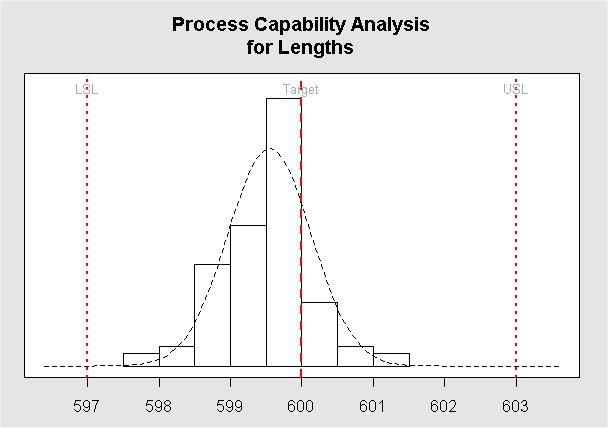
\includegraphics[scale=0.55]{image/ExamQ4hist}
	\end{center}
	\newpage
	%
	%Lengths = Values
	%
	%obj <- qcc(Lengths, type="xbar")
	%
	%process.capability(obj, spec.limits=c(597,603))


\subsubsection*{Question 5 Part C (12 Marks)}
% \subsection*{Question 47 - Nelson Rules for Control Charts}
The \textbf{Nelson Rules} are a set of eight decision rules for detecting ``out-of-control" or non-random conditions on control charts. These rules are applied to a control chart on which the magnitude of some variable is plotted against time. The rules are based on the mean value and the standard deviation of the samples.\\

\begin{itemize}
	\item[(i)] ($4 \times 3$ Marks) Discuss any four of these rules, and how they would be used to detect ``out of control" processes. Support your answer with sketch.
\end{itemize}

\bigskip 
\begin{framed}
	\noindent \textit{In your answer, you may make reference to the following properties of the Normal Distribution. Consider the random variable $X$ distributed as
		\[X \sim \mathcal{N}(\mu,\sigma^2)\]
		where $\mu$ is the mean and $\sigma^2$ is the variance of an random variable $X$.}
	\begin{itemize}
		\item $\Pr( \mu - 1\sigma \leq X \leq \mu + 1\sigma ) = 0.6827$
		\item $\Pr( \mu - 2\sigma \leq X \leq \mu + 2\sigma ) = 0.9545$
		\item $\Pr( \mu - 3\sigma \leq X \leq \mu + 3\sigma )= 0.9973$
		
	\end{itemize}
\end{framed}
\newpage
\subsection*{Critical Values for Dixon Q Test}
{
	\Large
	\begin{center}
		\begin{tabular}{|c|c|c|c|}
			\hline  N  & $\alpha=0.10$  & $\alpha=0.05$  & $\alpha=0.01$  \\ \hline
			3  & 0.941 & 0.970 & 0.994 \\ \hline
			4  & 0.765 & 0.829 & 0.926 \\ \hline
			5  & 0.642 & 0.710  & 0.821 \\ \hline
			6  & 0.560 & 0.625 & 0.740 \\ \hline
			7  & 0.507 & 0.568 & 0.680  \\ \hline
			8  & 0.468 & 0.526 & 0.634 \\ \hline
			9  & 0.437 & 0.493 & 0.598 \\ \hline
			10 & 0.412 & 0.466 & 0.568 \\ \hline
			11 & 0.392 & 0.444 & 0.542 \\ \hline
			12 & 0.376 & 0.426 & 0.522 \\ \hline
			13 & 0.361 & 0.410 & 0.503 \\ \hline
			14 & 0.349 & 0.396 & 0.488 \\ \hline
			15 & 0.338 & 0.384 & 0.475 \\ \hline
			16 & 0.329 & 0.374 & 0.463 \\ \hline
		\end{tabular} 
	\end{center}
}
\subsection*{Two Way ANOVA}
\[MS_A = c \times S^2_r\]
\[MS_B = r \times S^2_c\]

\subsection*{Control Limits for Control Charts}

 \[ \bar{\bar{x}} \pm 3\frac{\bar{s}}{c_4\sqrt{n}}\]

 \[ \bar{s} \pm 3\frac{c_5\bar{s}}{c_4}\]

 \[\left[ \bar{R}D_3, \bar{R}D_4\right]\]

\subsection*{Process Capability Indices}
\[ \hat{C}_p = \frac{\mbox{USL} - \mbox{LSL}}{6s}\]

\[ \hat{C}_{pk} = \mbox{min} \left[\frac{\mbox{USL} - \bar{x}}{3s},\frac{\bar{x} - \mbox{LSL}}{3s} \right] \]

\[ \hat{C}_{pm} = \frac{\mbox{USL} - \mbox{LSL}}{6\sqrt{s^2+(\bar{x}-T)^2}}\]
\bigskip
%\subsection*{2^3 Design: Main Effect}
%
%\[X= \frac{1}{4n} \left[ x + xy + xz + xyz - (1) - y - z - yz \right]\]
%\bigskip
\subsection*{$2^3$ Design: Interaction Effects}

\[ AB = \frac{1}{4n} \left[ abc - bc + ab - b - ac + c - a + (1) \right] \]

\[ AC = \frac{1}{4n} \left[ (1) - a + b - ab -c + ac - bc + abc \right] \]

\[ BC = \frac{1}{4n} \left[ (1) + a - b - ab - c - ac + bc + abc \right] \]

\[ABC = \frac{1}{4n} \left[ abc - bc - ac + c - ab + b +  a - (1) \right] \]

\bigskip

\subsection*{Factorial Design: Sums of Squares}

\[\mbox{Effect} =  \frac{\mbox{Contrast}}{4n}\]

\[\mbox{Sums of Squares} =  \frac{\mbox{(Contrast)}^2}{8n}\]

%------------------------------------------------------------------------ %
\Large{
\subsection*{Factors for Control Charts}
\begin{tabular}{|c|c|c|c|c|c|c|}
\hline
Sample Size (n) 	&	c4 	&	c5 	&	d2 	&	d3 	&	D3 	&	D4	\\	\hline
2	&	0.7979	&	0.6028	&	1.128	&	0.853	&	0	&	3.267	\\	
3	&	0.8862	&	0.4633	&	1.693	&	0.888	&	0	&	2.574	\\	
4	&	0.9213	&	0.3889	&	2.059	&	0.88	&	0	&	2.282	\\	
5	&	0.9400	&	0.3412	&	2.326	&	0.864	&	0	&	2.114	\\	
6	&	0.9515	&	0.3076	&	2.534	&	0.848	&	0	&	2.004	\\	
7	&	0.9594	&	0.282	&	2.704	&	0.833	&	0.076	&	1.924	\\	
8	&	0.9650	&	0.2622	&	2.847	&	0.82	&	0.136	&	1.864	\\	
9	&	0.9693	&	0.2459	&	2.970	&	0.808	&	0.184	&	1.816	\\	
10	&	0.9727	&	0.2321	&	3.078	&	0.797	&	0.223	&	1.777	\\	
11	&	0.9754	&	0.2204	&	3.173	&	0.787	&	0.256	&	1.744	\\	
12	&	0.9776	&	0.2105	&	3.258	&	0.778	&	0.283	&	1.717	\\	
13	&	0.9794	&	0.2019	&	3.336	&	0.770	&	0.307	&	1.693	\\	
14	&	0.9810	&	0.1940	&	3.407	&	0.763	&	0.328	&	1.672	\\	
15	&	0.9823	&	0.1873	&	3.472	&	0.756	&	0.347	&	1.653	\\	
16	&	0.9835	&	0.1809	&	3.532	&	0.750	&	0.363	&	1.637	\\
17	&	0.9845	&	0.1754	&	3.588	&	0.744	&	0.378	&	1.622	\\
18	&	0.9854	&	0.1703	&	3.64	&	0.739	&	0.391	&	1.608	\\
19	&	0.9862	&	0.1656	&	3.689	&	0.734	&	0.403	&	1.597	\\
20	&	0.9869	&	0.1613	&	3.735	&	0.729	&	0.415	&	1.585	\\
21	&	0.9876	&	0.1570	&	3.778	&	0.724	&	0.425	&	1.575	\\
22	&	0.9882	&	0.1532	&	3.819	&	0.720	&	0.434	&	1.566	\\
23	&	0.9887	&	0.1499	&	3.858	&	0.716	&	0.443	&	1.557	\\
24	&	0.9892	&	0.1466	&	3.895	&	0.712	&	0.451	&	1.548	\\
25	&	0.9896	&	0.1438	&	3.931	&	0.708	&	0.459	&	1.541	\\
\hline
\end{tabular}
} % End Large Font
\end{document}




